%% This is file `prletters-template.tex',
%%
%% Copyright 2013 Elsevier Ltd
%%
%% This file is part of the 'Elsarticle Bundle'.
%% ---------------------------------------------
%%
%% It may be distributed under the conditions of the LaTeX Project Public
%% License, either version 1.2 of this license or (at your option) any
%% later version.  The latest version of this license is in
%%    http://www.latex-project.org/lppl.txt
%% and version 1.2 or later is part of all distributions of LaTeX
%% version 1999/12/01 or later.
%%
%% The list of all files belonging to the 'Elsarticle Bundle' is
%% given in the file `manifest.txt'.
%%
%% Template article for Elsevier's document class `elsarticle'
%% with harvard style bibliographic references
%%
%% $Id: prletters-template-with-authorship.tex 69 2013-07-15 10:15:25Z rishi $
%%
%% This template has no review option
%%
%% Use the options `twocolumn,final' to obtain the final layout
\documentclass[times,twocolumn,final,authoryear]{elsarticle}

%% Stylefile to load PR Letters template
\usepackage{prletters}
\usepackage{framed,multirow}

%% The amssymb package provides various useful mathematical symbols
\usepackage{amssymb}
\usepackage{latexsym}

% Following three lines are needed for this document.
% If you are not loading colors or url, then these are
% not required.
\usepackage{url}
\usepackage{xcolor}
\definecolor{newcolor}{rgb}{.8,.349,.1}

\newcommand{\T}{^{\ensuremath{\mathsf{T}}}}           % transpose
\newcommand{\mrsid}{{\sc \texttt{Mr}.~\texttt{Sid}}}
\newcommand{\argmax}{\operatornamewithlimits{argmax}}
\newcommand{\argmin}{\operatornamewithlimits{argmin}}
\newcommand{\diag}{\operatornamewithlimits{diag}}


\journal{Pattern Recognition Letters}

\begin{document}

\thispagestyle{empty}

\begin{table*}[!th]

\begin{minipage}{.9\textwidth}
\baselineskip12pt
\ifpreprint
  \vspace*{1pc}
\else
  \vspace*{-6pc}
\fi

\noindent {\LARGE\itshape Pattern Recognition Letters}
\vskip6pt

\noindent {\Large\bfseries Authorship Confirmation}

\vskip1pc


{\bf Please save a copy of this file, complete and upload as the
``Confirmation of Authorship'' file.}

\vskip1pc

As corresponding author
I, \underline{ Shaojie Chen },
hereby confirm on behalf of all authors that:

\vskip1pc

\begin{enumerate}
\itemsep=3pt
\item This manuscript, or a large part of it, \underline {has not been
published,  was not, and is not being submitted to} any other journal.

\item If \underline {presented} at or \underline {submitted} to or
\underline  {published }at a conference(s), the conference(s) is (are)
identified and  substantial \underline {justification for
re-publication} is presented  below. A \underline {copy of
conference paper(s) }is(are) uploaded with the  manuscript.

\item If the manuscript appears as a preprint anywhere on the web, e.g.
arXiv,  etc., it is identified below. The \underline {preprint should
include a  statement that the paper is under consideration at Pattern
Recognition  Letters}.

\item All text and graphics, except for those marked with sources, are
\underline  {original works} of the authors, and all necessary
permissions for  publication were secured prior to submission of the
manuscript.

\item All authors each made a significant contribution to the research
reported  and have \underline {read} and \underline {approved} the
submitted  manuscript.
\end{enumerate}

Signature\underline{: Shaojie Chen} Date\underline{: 06/19/2016}
\vskip1pc

\rule{\textwidth}{2pt}
{\bf List any pre-prints: arXiv}
\vskip1pc


\rule{\textwidth}{2pt}
{\bf Relevant Conference publication(s) (submitted, accepted, or published): NA}
\vskip1pc

{\bf Justification for re-publication: NA}

\end{minipage}
\end{table*}


\begin{table*}[!t]
\ifpreprint\else\vspace*{-15pc}\fi

\section*{Research Highlights (Required)}
\fboxsep=6pt
\fbox{
\begin{minipage}{.95\textwidth}
It should be short collection of bullet points that convey the core
findings of the article. It should  include 3 to 5 bullet points
(maximum 85 characters, including spaces, per bullet point.)
\vskip1pc
\begin{itemize}

 \item

 \item

 \item

 \item

 \item

\end{itemize}
\vskip1pc
\end{minipage}
}

\end{table*}

\clearpage


\ifpreprint
  \setcounter{page}{1}
\else
  \setcounter{page}{1}
\fi

\begin{frontmatter}

\title{An M-estimator for reduced-rank system identification}

\author[1]{Shaojie \snm{Chen}\corref{cor1}}
\cortext[cor1]{Corresponding author:
  Tel.: +1-410-409-8132;}
\ead{pzcsj76@gmail.com}
\author[2]{Kai \snm{Liu}}
\author[3]{Yuguang \snm{Yang}}
\author[1]{Yuting \snm{Xu}}
\author[4]{Seonjoo \snm{Lee}}
\author[1]{Martin \snm{Lindquist}}
\author[1]{Brian \snm{Caffo}}
\author[5,6]{Joshua T. \snm{Vogelstein}}

\address[1]{\small Dept. of Biostatistics, Johns Hopkins Bloomberg School of Public Health, USA}
\address[2]{Dept. of Neuroscience, Johns Hopkins University, USA}
\address[3]{Dept. of Chemical and Biomolecular Engineering, Johns Hopkins University, USA}
\address[4]{Dept. of Psychiatry and Department of Biostatistics, Columbia University, USA}
\address[5]{Child Mind Institute, USA}
\address[6]{Dept. of Biomedical Engineering and Institute for Computational Medicine, Johns Hopkins University, USA}

\received{1 May 2013}
\finalform{10 May 2013}
\accepted{13 May 2013}
\availableonline{15 May 2013}
\communicated{S. Sarkar}


\begin{abstract}
High-dimensional time-series data from a wide variety of domains, such as neuroscience, are being generated every day. Fitting statistical models to such data, to enable parameter estimation and time-series prediction, is an important computational primitive. Existing methods, however, are unable to cope with the high-dimensional nature of these data, due to both computational and statistical reasons.  We mitigate both kinds of issues by proposing an M-estimator for Reduced-rank System IDentification (\mrsid). A combination of low-rank approximations, $\ell_1$ and $\ell_2$ penalties, and some numerical linear algebra tricks, yields an estimator that is computationally efficient and numerically stable.  Simulations and real data examples demonstrate the usefulness of this approach in a variety of problems.  In particular, we demonstrate that \mrsid~can accurately estimate spatial filters, connectivity graphs, and time-courses from native resolution functional magnetic resonance imaging data. \mrsid~therefore enables big time-series data to be analyzed using standard methods, readying the field for further generalizations including nonlinear and non-Gaussian state-space models.

\end{abstract}

\begin{keyword}
\MSC 41A05\sep 41A10\sep 65D05\sep 65D17
\KWD Keyword1\sep Keyword2\sep Keyword3

%% MSC codes here, in the form: \MSC code \sep code
%% or \MSC[2008] code \sep code (2000 is the default)
\end{keyword}

\end{frontmatter}

%\linenumbers

%% main text
\section{Introduction}

%\begin{itemize}
%\item proposed a penalized linear dynamical system model (\mrsid)
%\item designed an expectation-maximization algorithm to solve the proposed model
%\item used the model for neuroimage data analysis and explored the primary motor cortex of human brain
%\end{itemize}
High-dimensional  time-series data are becoming increasingly  abundant across a wide variety of domains, spanning economics \cite{Johansen1988}, neuroscience \citep{Friston2003a},   and cosmology \citep{Xie2013a}. Fitting statistical models to such data, to enable parameter estimation and time-series prediction, is an important computational primitive.
Linear dynamical system (LDS) models are amongst the most popular and powerful, because of their intuitive nature and ease of implementation \citep{Kalman1963}.   The famous Kalman Filter-Smoother is one of the most popular and powerful tools for time-series prediction with an LDS, given known parameters \citep{Kalman1960a}.
% * <stefaniejacinto@gmail.com> 2016-03-31T21:44:25.404Z:
%
% > Filter Smoother
%
% Edit to be consistent with whatever we decide for the term used earlier in the abstract (Filter-Smoother or Filter/Smoother)
%
% ^ <joshuav@gmail.com> 2016-05-12T03:59:31.456Z.
In practice, however, for many LDS's, the parameters are unknown and must be estimated in a process often called \emph{system identification} \citep{Ljung1998}.  To the best of our knowledge, currently there does not exist a methodology that provides parameter estimates and predictions from ultra-high-dimensional time-series data (e.g. $p > 10$,$000$).
% * <stefaniejacinto@gmail.com> 2016-04-03T00:48:26.597Z:
%
% > system identification
%
% Discuss: I removed "in this domain" after system identification because I felt it was unnecessary. But is there a specific reason why that needs to be mentioned?
%
% ^ <joshuav@gmail.com> 2016-05-12T03:59:54.536Z.

The challenges associated with high-dimensional time-series estimation and prediction are multifold.  First, na\"ively, such models include dense $p \times p$ matrices, which are often too large to store, much less invert in memory.  Several recent efforts to invert large sparse matrices using a series of computational tricks show promise, though they are still extremely computationally expensive  \citep{Hsieh2013, Banerjee2013a}.
% * <stefaniejacinto@gmail.com> 2016-03-31T21:49:30.704Z:
%
% > such naive
%
% Discuss: This was originally "naively such models...", need to confirm if this language is equivalent.
%
% ^ <joshuav@gmail.com> 2016-05-12T04:00:40.851Z.
Second, estimators behave poorly due to numerical instability.
Reduced-rank LDS models can partially address this problem by reducing the number of latent states.  \citep{CHEN1989}.  However, without further constraints, the dimensionality of the latent states would be reduced to such an extent  that it would significantly decrease the predictive capacity of the resulting model.  Third, even after addressing these problems, the time to compute all the necessary quantities can be overly burdensome. Distributed memory implementations, such as those built with Spark, might help overcome this problem. However, it would lead to additional costs and set-up burden, as it would require a Spark cluster \citep{Zaharia2010}.
% * <stefaniejacinto@gmail.com> 2016-04-03T00:47:14.625Z:
%
% > However, without further constraints, the dimensionality of the latent states would be reduced to such an extent  that it would significantly decrease the predictive capacity of the resulting model.
%
% Discuss: I reworded this sentence to make it clearer, need to confirm it now reflects what the authors intended.
%
% ^ <joshuav@gmail.com> 2016-05-12T04:01:00.944Z.
% * <stefaniejacinto@gmail.com> 2016-03-31T21:52:32.570Z:
%
% > CHEN
%
% Is there a reason for this reference to be in all capital letters? It looks like this is the same Chen who is the first author of this paper. But I'm pretty sure that we need to have a consistent format for all the references.
%
% ^ <joshuav@gmail.com> 2016-05-12T04:06:49.405Z.

We address all three of these issues with our M-estimator for Reduced-rank  System IDentification (\mrsid).  By assuming the dimensionality of the latent state space is small (i.e. reduced-rank), relative to the observed space dimensionality, we can significantly improve computational tractability and estimation accuracy. By further penalizing the estimators, with $\ell_1$ and/or $\ell_2$ penalties, via utilizing prior knowledge on the structure of the parameters, we gain further estimation accuracy in this high-dimensional but relatively low-sample size regime.  Finally, by employing several numerical linear algebra tricks, we can reduce the computational burden significantly.
% * <stefaniejacinto@gmail.com> 2016-03-31T22:01:38.412Z:
%
% > and
%
% Need more clarification on this sentence. Is the "prior knowledge" used for the l1 and l2 penalties? Or does it refer to other things? This would affect how we'd rewrite this sentence.
%
% ^ <joshuav@gmail.com> 2016-05-12T04:08:31.470Z.
% * <stefaniejacinto@gmail.com> 2016-03-31T21:58:55.027Z:
%
% > ambient
%
% I don't think we need "or observed" here. We are already clarifying another term earlier in the sentence, so it would be awkward to do the same to explain ambient. Would everyone understand what we mean when we say "ambient"? If yes, maybe we don't need to say "observed".
%
% ^ <joshuav@gmail.com> 2016-05-12T04:09:21.456Z.
% * <stefaniejacinto@gmail.com> 2016-03-31T21:56:56.140Z:
%
% > Reduced-Rank  System Identification
%
% Edit to be consistent with whatever we decide for the term used earlier in the abstract
%
% ^ <joshuav@gmail.com> 2016-05-12T04:09:45.654Z.

These three techniques combined enable us to obtain highly accurate estimates in a variety of simulation settings.  \mrsid~is, in fact, a generalization of the now classic Baum-Welch expectation maximization algorithm, commonly used for system identification in much lower dimensional linear dynamical systems \citep{rabiner1989tutorial}. We show numerically that the hyperparameters can be selected to minimize prediction error on held-out data.  Finally, we use \mrsid~to estimate functional connectomes from the motor cortex.  \mrsid~enables us to estimate the regions, rather than imposing some prior parcellation on the data, as well as estimate sparse connectivity between regions.  \mrsid~reliably estimates these connectomes, as well as predicts the held-out time-series data.  To our knowledge, this is the first time a single unified approach has been used to estimate partitions and functional connectomes directly from the high-dimensional data.
% * <stefaniejacinto@gmail.com> 2016-03-31T22:04:07.548Z:
%
% > selected to minimize
%
% Discuss with client: is this what the author intended to say?
%
% ^ <joshuav@gmail.com> 2016-05-12T04:33:19.678Z.

This work presents a new analysis of a model which has only been implemented in low-dimensional settings,
and paves the way for high-dimensional implementation. Though primitive, it is a first step for essentially any high-dimensional time series analysis, control system identification, and spatiotemporal analysis. To enable extensions, generalizations, and additional applications, the code for the core functions and generating each of the figures is freely available on Github (\url{https://github.com/shachen/PLDS/}).
% * <stefaniejacinto@gmail.com> 2016-03-31T22:06:44.365Z:
%
% > functions
%
% Do we really need to say "functions"? Aren't functions part of the overall code?
%
% ^ <joshuav@gmail.com> 2016-05-12T04:34:17.550Z.


\section{The first page}
Avoid using abbreviations in the title. Next, list all authors with
their first names or initials and surnames (in that order). Indicate
the author for correspondence (see elsarticle documentation).

Present addresses can be inserted as footnotes. After having listed all
authors' names, you should list their respective affiliations. Link
authors and affiliations using superscript lower case letters.

\subsection{The Abstract}
An Abstract is required for every paper; it should succinctly summarize
the reason for the work, the main findings, and the conclusions of the
study. The abstract should be no longer than 200 words. Do not include
artwork, tables, elaborate equations or references to other parts of
the paper or to the reference listing at the end. ``Comment'' papers
are exceptions, where the commented paper should be referenced in full
in the Abstract.

The reason is that the Abstract should be understandable in itself to
be suitable for storage in textual information retrieval systems.

\textit{Example of an abstract: A biometric sample collected in an
uncontrolled outdoor environment varies significantly from its
indoor version. Sample variations due to outdoor environmental
conditions degrade the performance of biometric systems that
otherwise perform well with indoor samples. In this study, we
quantitatively evaluate such performance degradation in the case
of a face and a voice biometric system. We also investigate how
elementary combination schemes involving min-max or z
normalization followed by the sum or max fusion rule can
improve performance of the multi-biometric system. We use
commercial biometric systems to collect face and voice samples
from the same subjects in an environment that closely mimics the
operational scenario. This realistic evaluation on a dataset of
116 subjects shows that the system performance degrades in
outdoor scenarios but by multimodal score fusion the
performance is enhanced by 20\%. We also find that max rule
fusion performs better than sum rule fusion on this dataset. More
interestingly, we see that by using multiple samples of the same
biometric modality, the performance of a unimodal system can
approach that of a multimodal system.}

\section{The main text}

Please divide your article into (numbered) sections (You can find the
information about the sections at
\url{http://www.elsevier.com/wps/find/journaldescription.cws_home/505619/authorinstructions}).
Ensure that all tables, figures and schemes are cited in the text in
numerical order. Trade names should have an initial capital letter, and
trademark protection should be acknowledged in the standard fashion,
using the superscripted characters for trademarks and registered
trademarks respectively. All measurements and data should be given in
SI units where possible, or other internationally accepted units.
Abbreviations should be used consistently throughout the text, and all
nonstandard abbreviations should be defined on first usage
\citep{vanderGeeretal2000}.

\begin{table*}[!t]
\caption{\label{tab1}Summary of different works pertaining to face and
speech fusion}
\centering
\begin{tabular}{|p{2.25cm}|p{2cm}|l|p{4cm}|p{3cm}|p{2cm}|}
\hline
Study & Algorithm used & DB Size & Covariates of interest &
Top individual performance & Fusion\newline Performance\\
\hline
UK-BWG
(Mansfield et al.,
2001) &
Face, voice:\newline
Commercial & 200 & Time: 1--2 month\newline
separation (indoor) &
TAR$^*$ at 1\% FAR$^{\#}$\newline
Face: 96.5\%\newline
Voice: 96\%
& --\\
\hline
Brunelli
(Brunelli and
Falavigna, 1995) &
Face:\newline
Hierarchical\newline
correlation\newline
Voice:\newline
MFCC &
87 &
Time: 3 sessions, time\newline
unknown (indoor) &
Face:\newline
TAR = 92\% at\newline
4.5\% FAR\newline
Voice:\newline
TAR = 63\% at\newline
15\% FAR
&
TAR =98.5\%\newline
at 0.5\% FAR\\
\hline
Jain
(Jain et al., 1999)
&
Face:\newline
Eigenface\newline
Voice:\newline
Cepstrum\newline
Coeff. Based
&
50
&
Time: Two weeks (indoor)
&
TAR at 1\% FAR\newline
Face: 43\%\newline
Voice: 96.5\%\newline
Fingerprint: 96\%
&
Face $+$ Voice $+$\newline
Fingerprint $=$\newline
98.5\%\\
\hline
Sanderson
(Sanderson and
Paliwal, 2002)
&
Face: PCA\newline
Voice: MFCC &
43
& Time: 3 sessions (indoor)\newline
Noise addition to voice &
Equal Error Rate\newline
Face: 10\%\newline
Voice: 12.41\%
&
Equal Error\newline
Rate 2.86\% \\
\hline
Proposed study &
Face, voice:\newline
Commercial & 116 &
Location: Indoor and\newline
Outdoor (same day)\newline
Noise addition to eye\newline
coordinates
&
TARs at 1\% FAR\newline
Indoor-Outdoor\newline
Face: 80\%\newline
Voice: 67.5\%
&
TAR = 98\%\newline
at 1\% FAR\\
\hline
\multicolumn{6}{@{}l}{$^*$TAR--True Acceptance Rate\qquad
$^{\#}$ FAR--False Acceptance Rate}
\end{tabular}
\end{table*}


\subsection{Tables, figures and schemes}
Graphics and tables may be positioned as they should appear in the
final manuscript. Figures, Schemes, and Tables should be numbered.
Structures in schemes should also be numbered consecutively, for ease
of discussion and reference in the text. \textcolor{newcolor}{\bf
Figures should be maximum half a page size.}
All numbers and letters in figures and diagrams should be at least of
the same font size as that of the figure caption.

Depending on the
amount of detail, you can choose to display artwork in one column (20
pica wide) or across the page (42 pica wide). Scale your artwork in
your graphics program before incorporating it in your text. If the
artwork turns out to be too large or too small, resize it again in your
graphics program and re-import it. The text should not run along the
sides of any figure. This is an example for citation \citep{StrunkWhite1979}.

\begin{figure}[!t]
\centering
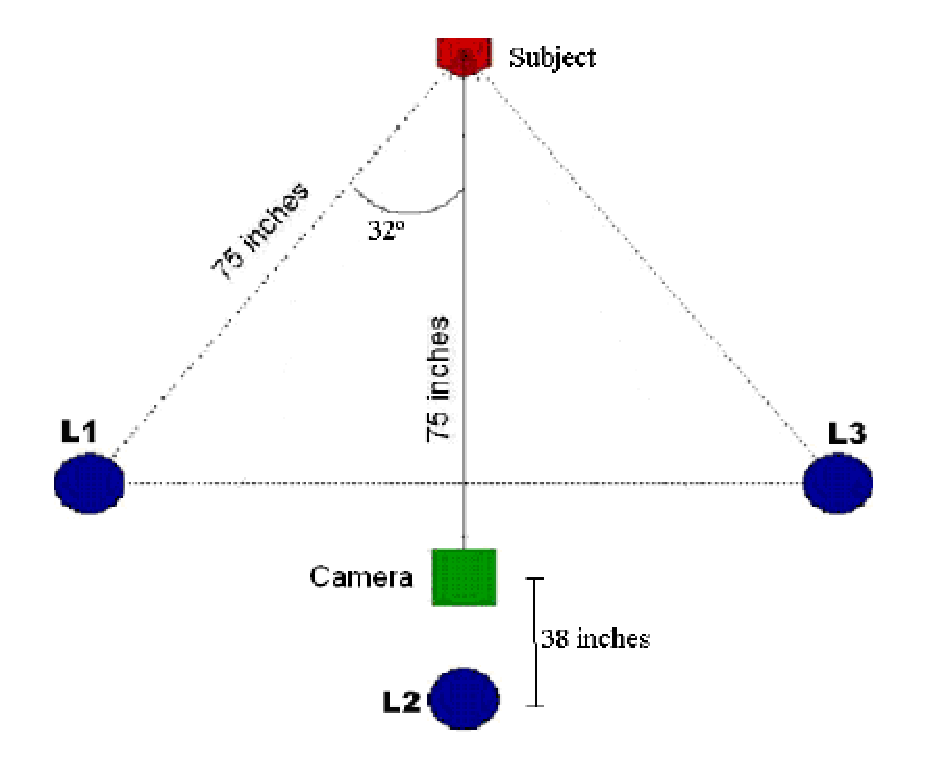
\includegraphics[scale=.5]{prletfig01}
\caption{Studio setup for capturing face images indoor. Three light
sources L1, L2, L3 were used in conjunction with normal office lights.}
\end{figure}

You might find positioning your artwork within the text difficult
anyway. In that case you may choose to place all artwork at the end of
the text and insert a marker in the text at the desired place. In any
case, please keep in mind that the placement of artwork may vary
somewhat in relation to the page lay-out \citep{MettamAdams1999}.

This can easily be achieved using \verb+endfloat.sty+ package. Please
refer the following documentation to use this package.
\makeatletter
\if@twocolumn
\begin{verbatim}
  http://mirrors.ctan.org/macros/latex/contrib/
  endfloat/endfloat.pdf
\end{verbatim}
\else
\begin{verbatim}
  http://mirrors.ctan.org/macros/latex/contrib/endfloat/endfloat.pdf
\end{verbatim}
\fi
\makeatother

\textcolor{newcolor}{\bf You should insert a caption for the figures
below the figures and for the tables the caption should be above the
tables.}

Please remember that we will always also need highresolution versions
of your artwork for printing, submitted as separate files in standard
format (i.e. TIFF or EPS), not included in the text document. Before
preparing your artwork, please take a look at our Web page:
\url{http://www.elsevier.com/locate/authorartwork}.


\subsection{Lists}

For tabular summations that do not deserve to be presented as
a table, lists are often used. Lists may be either numbered or
bulleted. Below you see examples of both.
\begin{enumerate}
\item The first entry in this list
\item The second entry
\begin{enumerate}
\item A subentry
\end{enumerate}
\item The last entry
\end{enumerate}
\begin{itemize}
\item A bulleted list item
\item Another one
\end{itemize}

\subsection{Equations}
Conventionally, in mathematical equations, variables and
anything that represents a value appear in italics.
All equations should be numbered for easy referencing. The number
should appear at the right margin.
\begin{equation}
S_{\rm pg}'=\frac{S_{\rm pg}-\min(S_{\rm pG})}
 {\max(S_{\rm pG}-\min(S_{\rm pG})}
\end{equation}
In mathematical expressions in running text ``/'' should be used for
division (not a horizontal line).

\section*{Acknowledgments}
Acknowledgments should be inserted at the end of the paper, before the
references, not as a footnote to the title. Use the unnumbered
Acknowledgements Head style for the Acknowledgments heading.

\section*{References}

Please ensure that every reference cited in the text is also present in
the reference list (and vice versa).

\section*{\itshape Reference style}

Text: All citations in the text should refer to:
\begin{enumerate}
\item Single author: the author's name (without initials, unless there
is ambiguity) and the year of publication;
\item Two authors: both authors' names and the year of publication;
\item Three or more authors: first author's name followed by `et al.'
and the year of publication.
\end{enumerate}
Citations may be made directly (or parenthetically). Groups of
references should be listed first alphabetically, then chronologically.

\bibliographystyle{model2-names}
\bibliography{reference}

\section*{Supplementary Material}

Supplementary material that may be helpful in the review process should
be prepared and provided as a separate electronic file. That file can
then be transformed into PDF format and submitted along with the
manuscript and graphic files to the appropriate editorial office.

\end{document}

%%
